\documentclass{beamer}

\usepackage[utf8]{inputenc}
\usepackage[russian]{babel}
\usepackage{cmap}

\mode<presentation> {
\usetheme{Madrid}
\setbeamertemplate{caption}[numbered]
}

\usepackage{graphicx} % Allows including images
\usepackage{booktabs} % Allows the use of \toprule, \midrule and \bottomrule in tables

\title[Теория распознавания образов]{Локализация и отслеживание лиц на изображении}

\author{Мартынов Семён}
\institute[СПбПУ]
{
Санкт-Петербургский политехнический университет Петра Великого \\
\medskip
\textit{semen.martynov@gmail.com}
}
\date{\today}

\begin{document}

\begin{frame}
\titlepage
\end{frame}

\begin{frame}
\frametitle{Содержание}
\tableofcontents
\end{frame}

%------------------------------------------------
\section{Базовые понятия}
%------------------------------------------------

\begin{frame}
\frametitle{Базовые понятия}
\begin{block}{Обнаружение лица}
Технология, определяющая наличие (иногда количество) лиц на цифровом изображении.
\end{block}

\begin{block}{Локализация лица}
Технология, определяющая положение лица на цифровом изображении (участке изображения), заведомо содержащем ровно одно лицо.
\end{block}

\begin{block}{Отслеживание лица}
Технология, определяющая положение лица в текущем кадре видео, и его смещение относительно предыдущего кадра.
\end{block}
\end{frame}

%------------------------------------------------

\begin{frame}
\frametitle{Пример автоматического обнаружения лиц}

\begin{figure}
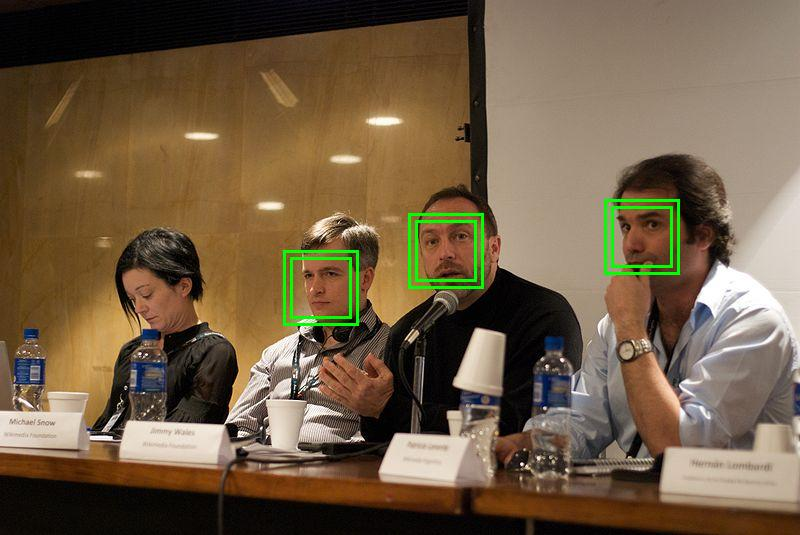
\includegraphics[scale=0.35]{res/img01}
\caption{Автоматическое обнаружение лиц при помощи OpenCV}
\end{figure}
\end{frame}

%------------------------------------------------
\section{Основы распознавания лиц}
%------------------------------------------------

\begin{frame}
\frametitle{Задачи обнаружения и распознавания лиц}

\begin{enumerate}
\item Задача обнаружения лиц (face detection)
    \begin{itemize}
    \item Охранные системы
    \item Автофокусировка
    \item Содержательная индексация базы изображений
    \end{itemize}
\pause
\item Задача распознавания лиц (Face Recognition)
    \begin{itemize}
    \item "Умные" охранные системы
    \item MOOC (Coursera)
    \item Верификация кредитных карточек
    \item Криминалистическая экспертиза
    \item Телеконференции
    \item Интерфейс человек-компьютер (Пример: SAMSUNG)
    \end{itemize}
\end{enumerate}
\end{frame}

%------------------------------------------------

\begin{frame}
\frametitle{Классы систем обнаружения лиц}

\begin{enumerate}
\item ручная - требует наличия оператора (офицер пограничной службы сравнивает фотографии из паспорта и реальное изображение человека);
\item автоматизированная - требует наличие оператора (доступ на охраняемый объект осуществляется по фотографии в документах и проксимити-карте);
\item автоматическая (задача установления личности осуществляется без участия человека).
\end{enumerate}
\end{frame}

%------------------------------------------------

\begin{frame}
\frametitle{Сложности построения автоматической системы}

\begin{enumerate}
\item сильно варьирующийся внешний вид лица у разных людей;
\item небольшое изменение ориентации лица относительно камеры приводит к серьезным изменениям изображения лица;
\item возможное присутствие индивидуальных особенностей (усы, бороды, очки, морщины и так далее);
\item изменение выражения лица (шум от эмоций);
\item часть лица может быть невидима (закрыта другими предметами) на изображении;
\item условия съемки (освещение, цветовой баланс камеры, искажения изображения, привносимые оптикой системы, качество изображения). 
\end{enumerate}
\end{frame}

%------------------------------------------------
\section{Эмпирические алгоритмы распознавания лиц}
%------------------------------------------------

\begin{frame}
\frametitle{Эмпирические алгоритмы распознавания лиц}

Основная идея - повторить работу человеческого мозга.

\begin{enumerate}
\item распознавание сверху-вниз -- принцип шаблона (производится описание свойств различных областей лица и их возможного взаимного расположения, а потом осуществляется проверка каждой из областей изображения на соответствие заданному шаблону);
\item Распознавание снизу-вверх -- инвариантные свойства (обнаружение и анализ элементов, инвариантных относительно условий съемки, которые характерны для изображения лица);
\end{enumerate}

\end{frame}

%------------------------------------------------
\subsection{Обнаружение характерных элементов и особенностей (features)}
%------------------------------------------------

\begin{frame}
\frametitle{Обнаружение характерных элементов и особенностей\\(features)}

\begin{itemize}
    \item \textbf{Края (edges)} -- резкие переходы яркости. Края обычно соответствуют границам объектов на изображении.
    \item \textbf{Яркость}. Области изображения, соответствующие чертам лица, зачастую темнее, чем окружающая их кожа.
    \item \textbf{Цвет} - цвет кожи разных людей занимает достаточно небольшую ограниченную подобласть цветового пространства (даже при рассмотрении цветов кожи различных рас)
    \item \textbf{Характерная форма черт лица} -- использование жестких или деформируемых шаблонов для обнаружения черт лица (например, глаз). 
\end{itemize}

\end{frame}
%------------------------------------------------
\begin{frame}
\frametitle{Обнаружение характерных элементов и особенностей\\(features)}

\begin{figure}
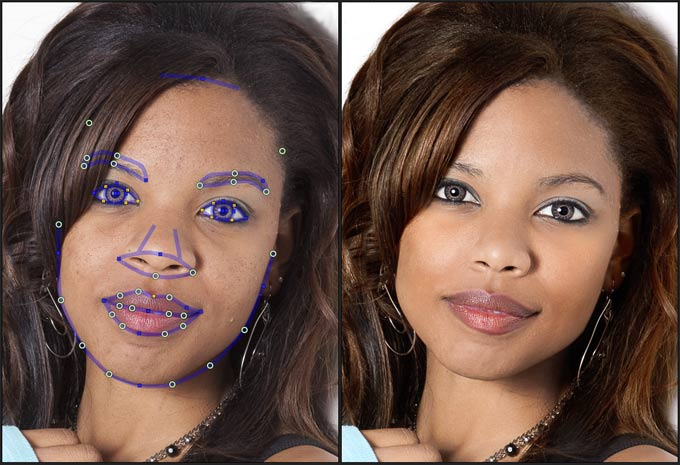
\includegraphics[scale=0.35]{res/img02}
\caption{Использование шаблонов для обнаружения черт лица}
\end{figure}

\end{frame}

%------------------------------------------------
\subsection{Комплексная проверка (complex test)}
%------------------------------------------------

\begin{frame}
\frametitle{Комплексная проверка\\(complex test)}

Основная идея в том, что обнаруживать элементы (глаза, нос, рот) легче, чем всё лицо. После этого нужно провести анализ их взаимного расположения с целью определения, могут ли они образовывать человеческое лицо.
\bigskip

Проверка соотношения обнаруженных признаков лица может быть основана на статистике взаимного расположения признаков.

\end{frame}
%------------------------------------------------
\begin{frame}
\frametitle{Комплексная проверка\\(complex test)}

\begin{figure}
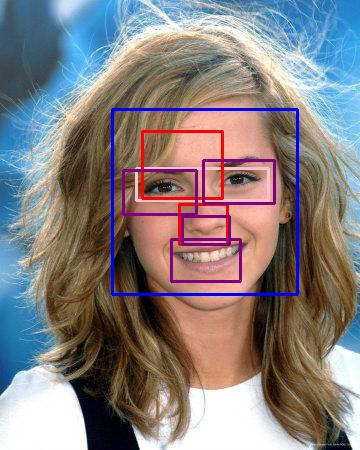
\includegraphics[scale=0.55]{res/img03}
\caption{Анализ взаимного расположения элементов лица}
\end{figure}

\end{frame}

%------------------------------------------------
\section{Алгоритмы математической статистики и машинного обучения}
%------------------------------------------------

\begin{frame}
\frametitle{Алгоритмы математической статистики\\и машинного обучения}

Основная идея - постараться поставить изображению (или его фрагменту) в соответствие некоторым образом вычисленный вектор признаков, который используется для классификации изображений на два класса - лицо/не лицо.
\bigskip

Самый простой способ это использование каждого пикселя как компонента вектора (т.о. черно-белое изображение $n*m$ превращается в вектор пространства $R^{n*m}$)

\begin{itemize}
\item[-] Чрезвычайно высокая размерность пространства признаков.
\item[+] Используя все изображение целиком вместо вычисленных на его основе характеристик.
\item[+] отсутствие человеческого фактора.
\end{itemize}

\end{frame}
%----------------------------------------------

\begin{frame}
\frametitle{Алгоритмы математической статистики\\и машинного обучения}

\begin{figure}
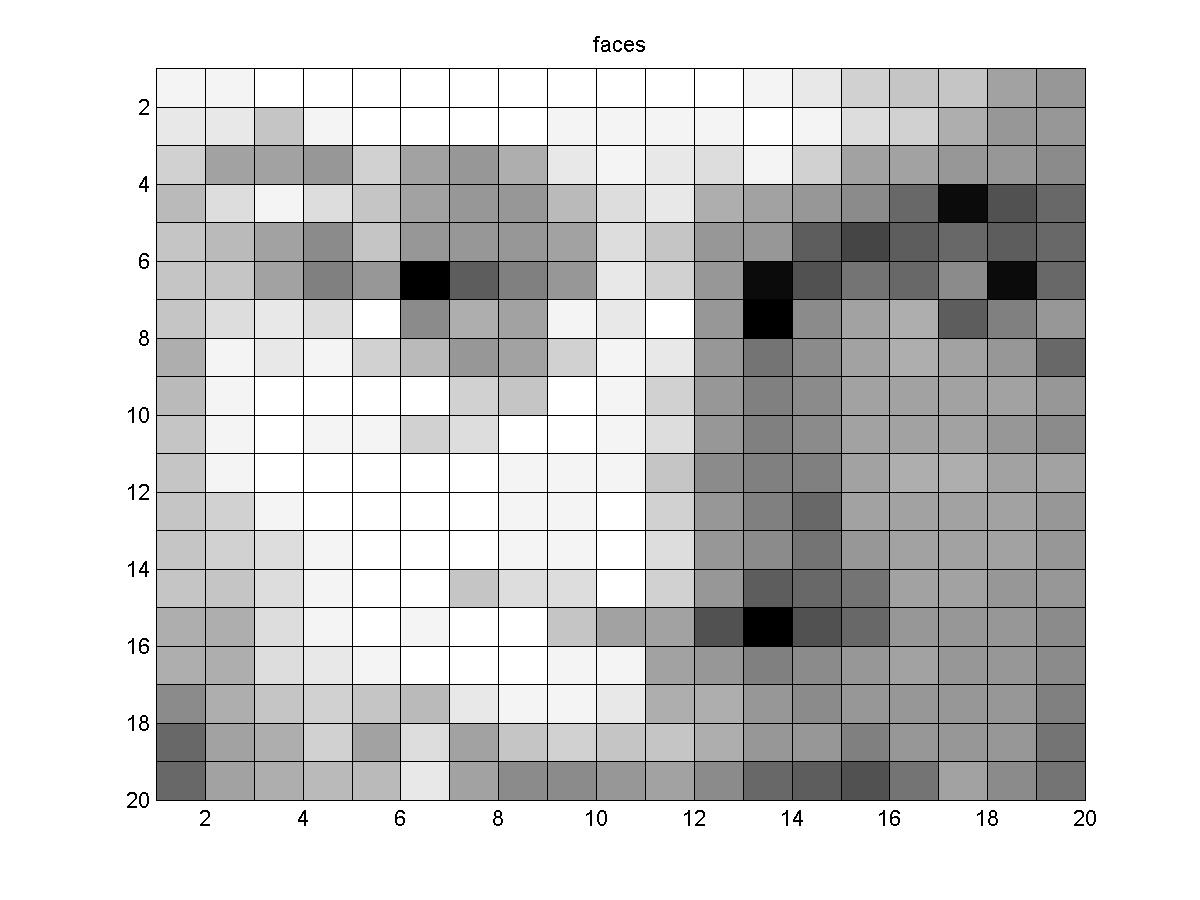
\includegraphics[scale=0.2]{res/img00}
\caption{Использование каждого пикселя как компонента вектора}
\end{figure}
\end{frame}

%------------------------------------------------
\subsection{Метод Главных Компонент (PCA)}
%----------------------------------------------

\begin{frame}
\frametitle{Метод Главных Компонент\\(Principal Components Analysis, PCA)}

Один из основных способов уменьшить размерность данных.
\bigskip

Вычисление главных компонент основывается на вычислении собственных векторов и собственных значений ковариационной матрицы, которая рассчитывается из изображения. 
\bigskip

Сумма главных компонент, умноженных на соответствующие собственные вектора, является реконструкцией изображения.
\bigskip

Основной недостаток – высокие требования к условиям съёмки изображений.

\end{frame}
%----------------------------------------------
\begin{frame}
\frametitle{Метод Главных Компонент\\(Principal Components Analysis, PCA)}

\begin{figure}
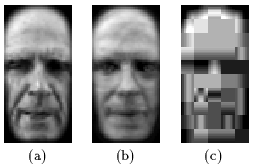
\includegraphics[scale=1]{res/img04}
\caption{а) выровненное изображение лица, б) реконструкция по 85-и главным компонентам, в) JPEG - реконструкция}
\end{figure}

\end{frame}

%------------------------------------------------
\subsection{Линейный Дискриминантный Анализ (LDA)}
%----------------------------------------------

\begin{frame}
\frametitle{Линейный Дискриминантный Анализ\\(Linear Discriminant Analysis, LDA)}

Основная идея - найти проекцию в пространство, в котором разница между различным классами объектов максимальна. Т.о. нужно получить максимально компактные кластера, соответствующие различным классам, удаленным на максимально возможное расстояние.
\bigskip

С помощью линейного дискриминантного анализа можно получить подпространство небольшой размерности, в котором кластеры изображений лиц и не-лиц пересекаются минимально.

\end{frame}
%----------------------------------------------

\begin{frame}
\frametitle{Линейный Дискриминантный Анализ\\(Linear Discriminant Analysis, LDA)}

\begin{figure}
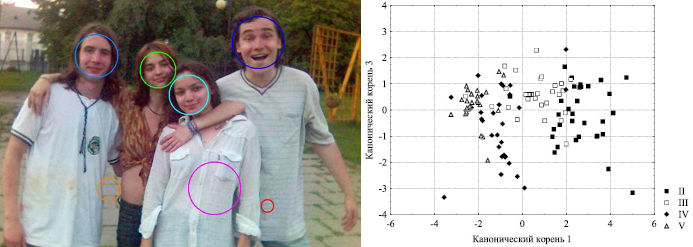
\includegraphics[scale=0.65]{res/img05}
\caption{Разделение кластеров}
\end{figure}

\end{frame}

%------------------------------------------------
\subsection{Метод Опорных Векторов (SVM)}
%----------------------------------------------

\begin{frame}
\frametitle{Метод Опорных Векторов\\(Support Vector Machines, SVM)}

Идея -- построить классификатор минимизирующий верхнюю оценку ожидаемой ошибки классификации (в том числе и для неизвестных объектов, не входивших в тренировочный набор). Применение метода опорных векторов к задаче обнаружения лица заключается в поиске гиперплоскости в признаковом пространстве, отделяющий класс изображений лиц от изображений "не-лиц". 

\end{frame}
%----------------------------------------------

\begin{frame}
\frametitle{Метод Опорных Векторов\\(Support Vector Machines, SVM)}

\begin{figure}
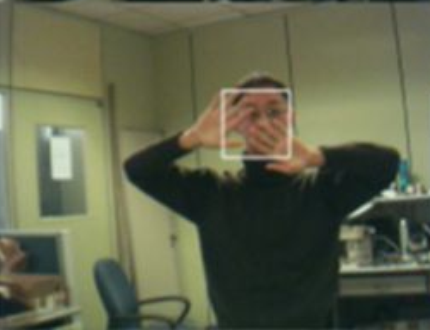
\includegraphics[scale=0.65]{res/img06}
\caption{Метод Опорных Векторов с высоким уровнем ожидаемой погрешности}
\end{figure}

\end{frame}

%------------------------------------------------
\subsection{Искусственные Нейронные Сети (NN)}
%----------------------------------------------

\begin{frame}
\frametitle{Искусственные Нейронные Сети\\(Neural Networks, NN)}

Для решения задач обнаружения лиц можно использовать сети различных конфигураций (построенных на различных элементах).
\bigskip

\begin{itemize}
\item[+] Возможность получения классификатора, хорошо моделирующего сложную функцию распределения изображений лиц.
\item[-] Необходимость в тщательной и кропотливой настройке нейросети для получения удовлетворительного результата.
\end{itemize}

\end{frame}
%----------------------------------------------

\begin{frame}
\frametitle{Искусственные Нейронные Сети\\(Support Vector Machines, SVM)}

\begin{figure}
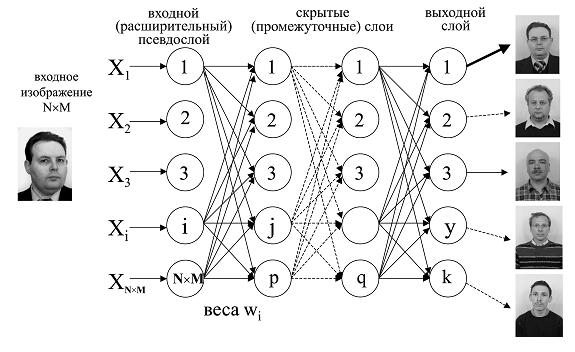
\includegraphics[scale=0.65]{res/img07}
\caption{Использование Искусственных Нейронных Сетей для определения похожести снимков}
\end{figure}

\end{frame}

%------------------------------------------------
\subsection{Разреженная сеть просеивающих элементов (SNoW)}
%----------------------------------------------

\begin{frame}
\frametitle{Разреженная сеть просеивающих элементов\\(Sparse Network of Winnows, SNoW)}

Реализация представляет из себя двухслойную сеть, входной слой которой состоит из узлов, каждый из которых соответствует некоторой характеристике входного изображения, а выходной состоит всего из двух узлов, каждый из которых соответствует распознаваемым классам изображений ("лицо", "не-лицо").
\bigskip

В качестве характеристик изображения используются флаги равенства определенным величинам среднего значения и дисперсии яркости в каждом из прямоугольных фрагментов изображения размером 1x1, 2x2, 4x4 и 10x10 (все изображения имеет размер 20x20 пикселей). Это дает пространство признаков размерности 135424.

\end{frame}
%----------------------------------------------

\begin{frame}
\frametitle{Разреженная сеть просеивающих элементов\\(Sparse Network of Winnows, SNoW)}

\begin{figure}
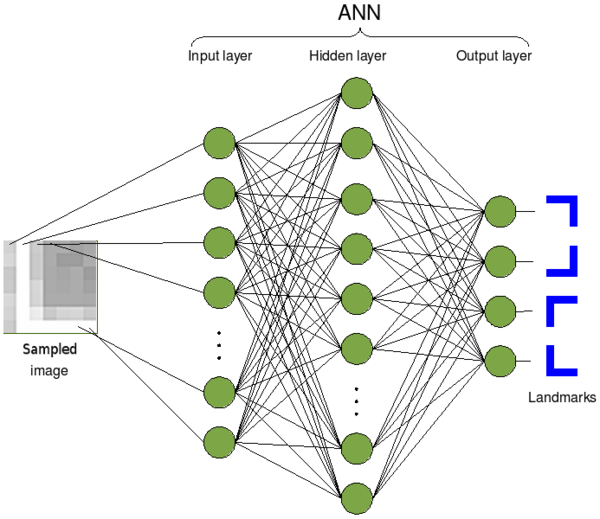
\includegraphics[scale=0.45]{res/img08}
\caption{Механизм работы разреженной сети просеивающих элементов}
\end{figure}

\end{frame}

%------------------------------------------------
\subsection{Скрытые Марковские Модели (HMM)}
%----------------------------------------------

\begin{frame}
\frametitle{Скрытые Марковские Модели\\(Hidden Markov Models, HMM)}

СММ относятся к классу стохастических моделей. Стохастические модели пытаются охарактеризовать только статистические свойства сигнала, не обладая информацией о его специфических свойствах.
\bigskip

Для применения СММ к задаче обнаружения лиц, нужно определить способ, которым изображения лица преобразуется в сигнал (набор последовательных наблюдений). Изображение лица можно естественным образом разделить на несколько горизонтальных областей: лоб, глаза, рот и подбородок. Лицо может быть представлено в виде сигнала, в котором передаются эти области в определенном порядке (обычно сверху-вниз, слева-направо).

\end{frame}
%----------------------------------------------

\begin{frame}
\frametitle{Скрытые Марковские Модели\\(Hidden Markov Models, HMM)}

\begin{figure}
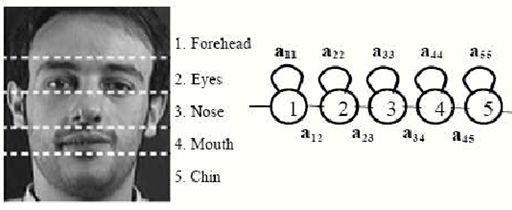
\includegraphics[scale=0.8]{res/img09}
\caption{Лицо в виде последовательности векторов наблюдений}
\end{figure}
\end{frame}

%------------------------------------------------
\subsection{Активные модели внешнего вида (AAM)}
%----------------------------------------------

\begin{frame}
\frametitle{Активные модели внешнего вида\\(Active Appearance Models, AAM)}

Модель позволяет моделировать изображения объектов, подверженных как жесткой (любая деформация, которая может быть представлена в виде композиции переноса, поворота и масштабирования) так и нежесткой деформации. Параметры модели выбираются автоматически, исходя из наиболее характерных деформаций формы и изменений текстуры, присутствующих в тренировочном наборе изображений объекта.
\bigskip

Активная модель внешнего вида лица задает изменения формы лица и его характерных черт (формы глаз, бровей, рта, носа, подбородка), а также возможные изменения текстуры лица. Для решения задачи обнаружения лица на изображении, делается попытка найти параметры (расположение, форма и текстура) AAM, которые задают изображение наиболее близкое к наблюдаемому.
\end{frame}
%----------------------------------------------

\begin{frame}
\frametitle{Активные модели внешнего вида\\(Active Appearance Models, AAM)}

\begin{figure}
\includegraphics[scale=0.5]{res/img10}
\caption{AAM на искаженном изображении лица}
\end{figure}
\end{frame}

%------------------------------------------------
\section{Вопросы}
%------------------------------------------------

\begin{frame}
\Huge{\centerline{Вопросы?}}
\end{frame}

%----------------------------------------------------------------------------------------

\end{document} 